% chap12_practical.tex - Putting it all together
% ============================================================================

\chapter{Practical Projects}
\label{chap:practical}

You've learned the pieces. Now let's put them together in complete, realistic projects. Each example demonstrates how the skills from previous chapters combine to solve actual scientific problems.

% ----------------------------------------------------------------------------
\section{Project 1: Calibration Curve Analysis}
\label{sec:project-calibration}

A common task: create a calibration curve from standards and use it to determine concentrations of unknown samples.

\begin{lstlisting}
import numpy as np
import pandas as pd
import matplotlib.pyplot as plt
from scipy.stats import linregress

# ============================================================
# Load and inspect data
# ============================================================
standards = pd.read_csv("standards.csv")
unknowns = pd.read_csv("unknowns.csv")

print("Standards:")
print(standards.head())
print("\nUnknowns:")
print(unknowns.head())

# ============================================================
# Calculate mean absorbance for each standard
# ============================================================
# Standards file has replicates
std_summary = standards.groupby("concentration")["absorbance"].agg(
    ["mean", "std", "count"]
).reset_index()
std_summary["sem"] = std_summary["std"] / np.sqrt(std_summary["count"])

# ============================================================
# Linear regression
# ============================================================
x = std_summary["concentration"].values
y = std_summary["mean"].values

result = linregress(x, y)
slope = result.slope
intercept = result.intercept
r_squared = result.rvalue ** 2

print(f"\nCalibration equation: A = {slope:.4f} * C + {intercept:.4f}")
print(f"R-squared: {r_squared:.6f}")

# ============================================================
# Create calibration plot
# ============================================================
fig, ax = plt.subplots(figsize=(8, 6))

# Plot standards with error bars
ax.errorbar(x, y, yerr=std_summary["sem"], fmt="ko",
            capsize=5, label="Standards")

# Plot regression line
x_line = np.linspace(0, x.max() * 1.1, 100)
y_line = slope * x_line + intercept
ax.plot(x_line, y_line, "r-", label=f"Fit: (*@$R^2$@*) = {r_squared:.4f}")

ax.set_xlabel("Concentration (M)")
ax.set_ylabel("Absorbance (AU)")
ax.set_title("Calibration Curve")
ax.legend()
ax.grid(True, alpha=0.3)

plt.tight_layout()
plt.savefig("calibration_curve.pdf")
\end{lstlisting}

\begin{center}
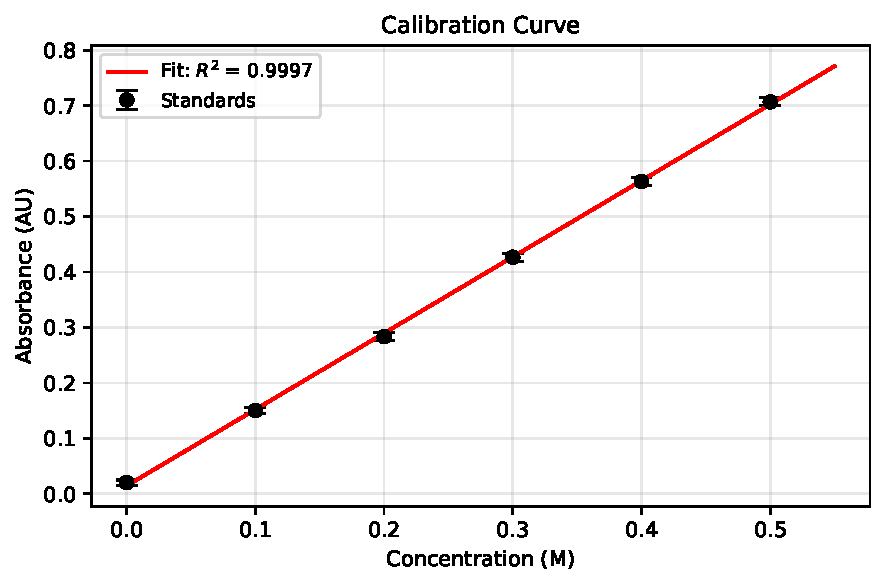
\includegraphics[width=0.75\textwidth]{figures/chap12/calibration_curve.pdf}
\end{center}

\begin{lstlisting}
# ============================================================
# Calculate unknown concentrations
# ============================================================
unknowns["concentration"] = (unknowns["absorbance"] - intercept) / slope

# Check if within calibration range
min_std = x.min()
max_std = x.max()
unknowns["in_range"] = (unknowns["concentration"] >= min_std) & \
                       (unknowns["concentration"] <= max_std)

# Flag samples outside range
outside_range = unknowns[~unknowns["in_range"]]
if len(outside_range) > 0:
    print(f"\nWarning: {len(outside_range)} samples outside calibration range")

# ============================================================
# Save results
# ============================================================
unknowns.to_csv("unknown_concentrations.csv", index=False)
print(f"\nResults saved. Processed {len(unknowns)} samples.")
\end{lstlisting}

% ----------------------------------------------------------------------------
\section{Project 2: Kinetics Data Analysis}
\label{sec:project-kinetics}

Analyze reaction kinetics data to determine rate constants and reaction order.

\begin{lstlisting}
import numpy as np
import pandas as pd
import matplotlib.pyplot as plt
from scipy.optimize import curve_fit

# ============================================================
# Load kinetics data
# ============================================================
data = pd.read_csv("kinetics_data.csv")
time = data["time_s"].values
concentration = data["concentration_M"].values

# ============================================================
# Define kinetic models
# ============================================================
def first_order(t, C0, k):
    """First-order decay: C = C0 * exp(-kt)"""
    return C0 * np.exp(-k * t)

def second_order(t, C0, k):
    """Second-order decay: 1/C = 1/C0 + kt"""
    return C0 / (1 + C0 * k * t)

# ============================================================
# Fit both models
# ============================================================
# First order
try:
    popt1, pcov1 = curve_fit(first_order, time, concentration)
    C0_1, k1 = popt1
    y_fit1 = first_order(time, *popt1)
    ss_res1 = np.sum((concentration - y_fit1)**2)
    ss_tot = np.sum((concentration - np.mean(concentration))**2)
    r2_1 = 1 - ss_res1/ss_tot
    print(f"First-order: k = {k1:.4f} (*@s$^{-1}$@*), (*@$R^2$@*) = {r2_1:.4f}")
except:
    print("First-order fit failed")

# Second order
try:
    popt2, pcov2 = curve_fit(second_order, time, concentration)
    C0_2, k2 = popt2
    y_fit2 = second_order(time, *popt2)
    ss_res2 = np.sum((concentration - y_fit2)**2)
    r2_2 = 1 - ss_res2/ss_tot
    print(f"Second-order: k = {k2:.4f} (*@M$^{-1}$s$^{-1}$@*), (*@$R^2$@*) = {r2_2:.4f}")
except:
    print("Second-order fit failed")

# ============================================================
# Determine best model
# ============================================================
if r2_1 > r2_2:
    best_model = "First-order"
    best_k = k1
    best_fit = y_fit1
else:
    best_model = "Second-order"
    best_k = k2
    best_fit = y_fit2

print(f"\nBest fit: {best_model}")

# ============================================================
# Create diagnostic plots
# ============================================================
fig, axes = plt.subplots(2, 2, figsize=(10, 8))

# Raw data with fits
ax1 = axes[0, 0]
ax1.plot(time, concentration, "ko", label="Data")
ax1.plot(time, y_fit1, "b-", label=f"1st order ((*@$R^2$@*)={r2_1:.3f})")
ax1.plot(time, y_fit2, "r--", label=f"2nd order ((*@$R^2$@*)={r2_2:.3f})")
ax1.set_xlabel("Time (s)")
ax1.set_ylabel("Concentration (M)")
ax1.legend()
ax1.set_title("Model Comparison")

# First-order linearization: ln(C) vs t
ax2 = axes[0, 1]
ax2.plot(time, np.log(concentration), "ko")
ax2.set_xlabel("Time (s)")
ax2.set_ylabel("ln(C)")
ax2.set_title("First-Order Test")

# Second-order linearization: 1/C vs t
ax3 = axes[1, 0]
ax3.plot(time, 1/concentration, "ko")
ax3.set_xlabel("Time (s)")
ax3.set_ylabel("1/C ((*@M$^{-1}$@*))")
ax3.set_title("Second-Order Test")

# Residuals for best fit
ax4 = axes[1, 1]
residuals = concentration - best_fit
ax4.plot(time, residuals, "ko")
ax4.axhline(y=0, color="r", linestyle="--")
ax4.set_xlabel("Time (s)")
ax4.set_ylabel("Residual")
ax4.set_title(f"Residuals ({best_model})")

plt.tight_layout()
plt.savefig("kinetics_analysis.pdf")
\end{lstlisting}

\begin{center}
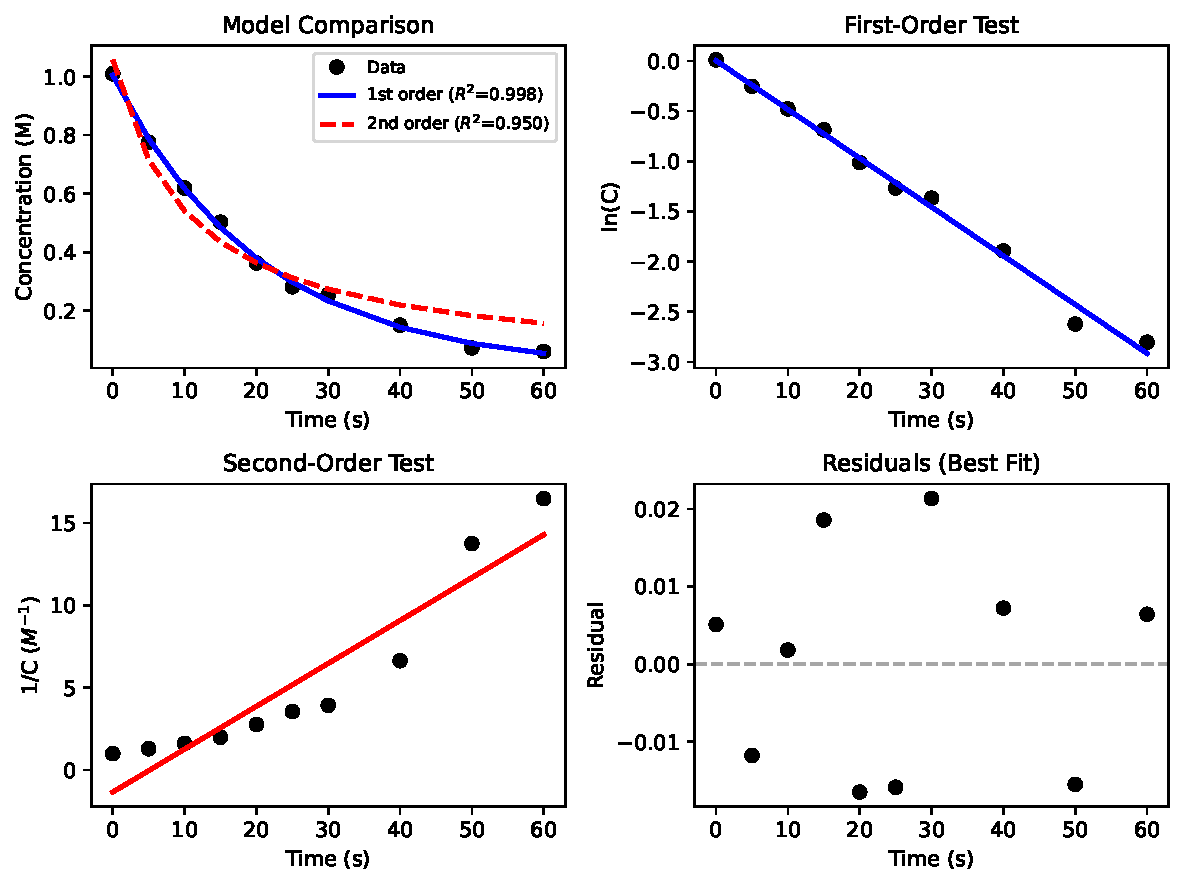
\includegraphics[width=0.85\textwidth]{figures/chap12/kinetics_analysis.pdf}
\end{center}

\begin{lstlisting}
# ============================================================
# Calculate half-life
# ============================================================
if best_model == "First-order":
    half_life = np.log(2) / best_k
else:
    half_life = 1 / (best_k * concentration[0])

print(f"Half-life: {half_life:.2f} s")
\end{lstlisting}

% ----------------------------------------------------------------------------
\section{Project 3: Batch Processing Spectra}
\label{sec:project-spectra}

Process multiple spectrum files: baseline correction, peak finding, and summary report.

\begin{lstlisting}
import numpy as np
import pandas as pd
import matplotlib.pyplot as plt
from pathlib import Path
from scipy.signal import find_peaks, savgol_filter

# ============================================================
# Setup
# ============================================================
data_folder = Path("spectra")
output_folder = Path("processed")
output_folder.mkdir(exist_ok=True)

results = []

# ============================================================
# Processing functions
# ============================================================
def load_spectrum(filepath):
    """Load spectrum from CSV file."""
    df = pd.read_csv(filepath)
    return df["wavelength"].values, df["absorbance"].values

def baseline_correct(absorbance, percentile=5):
    """Subtract baseline estimated from lowest values."""
    baseline = np.percentile(absorbance, percentile)
    return absorbance - baseline

def find_spectrum_peaks(wavelengths, absorbance, min_height=0.1):
    """Find peaks in spectrum."""
    peak_indices, properties = find_peaks(absorbance, height=min_height)
    peak_wavelengths = wavelengths[peak_indices]
    peak_heights = properties["peak_heights"]
    return list(zip(peak_wavelengths, peak_heights))

# ============================================================
# Process each file
# ============================================================
for filepath in sorted(data_folder.glob("*.csv")):
    print(f"Processing {filepath.name}...")

    # Load
    wavelengths, absorbance = load_spectrum(filepath)

    # Smooth
    abs_smooth = savgol_filter(absorbance, window_length=11, polyorder=3)

    # Baseline correct
    abs_corrected = baseline_correct(abs_smooth)

    # Find peaks
    peaks = find_spectrum_peaks(wavelengths, abs_corrected, min_height=0.05)

    # Record results
    sample_result = {
        "filename": filepath.name,
        "max_absorbance": np.max(abs_corrected),
        "num_peaks": len(peaks),
    }

    # Add first 3 peaks
    for i, (wl, height) in enumerate(peaks[:3]):
        sample_result[f"peak{i+1}_wavelength"] = wl
        sample_result[f"peak{i+1}_height"] = height

    results.append(sample_result)

    # Save processed spectrum
    processed = pd.DataFrame({
        "wavelength": wavelengths,
        "raw": absorbance,
        "smoothed": abs_smooth,
        "corrected": abs_corrected
    })
    processed.to_csv(output_folder / f"processed_{filepath.name}", index=False)

    # Create figure
    fig, ax = plt.subplots(figsize=(8, 5))
    ax.plot(wavelengths, absorbance, "gray", alpha=0.5, label="Raw")
    ax.plot(wavelengths, abs_corrected, "b-", label="Corrected")

    # Mark peaks
    for wl, height in peaks:
        ax.annotate(f"{wl:.0f}", xy=(wl, height), fontsize=8,
                   ha="center", va="bottom")

    ax.set_xlabel("Wavelength (nm)")
    ax.set_ylabel("Absorbance (AU)")
    ax.set_title(filepath.stem)
    ax.legend()

    plt.tight_layout()
    plt.savefig(output_folder / f"{filepath.stem}.png", dpi=150)
    plt.close()

# ============================================================
# Create summary
# ============================================================
summary = pd.DataFrame(results)
summary.to_csv(output_folder / "summary.csv", index=False)

print(f"\nProcessed {len(results)} files")
print(f"Results saved to {output_folder}")
print("\nSummary:")
print(summary[["filename", "max_absorbance", "num_peaks"]].to_string())
\end{lstlisting}

An example of processed output:

\begin{center}
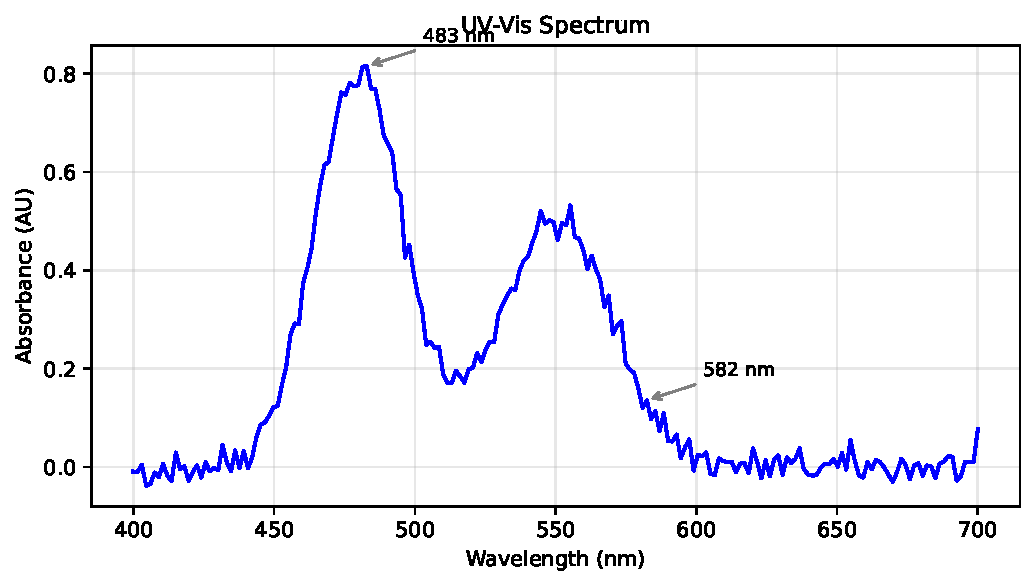
\includegraphics[width=0.75\textwidth]{figures/chap12/spectrum_example.pdf}
\end{center}

% ----------------------------------------------------------------------------
\section{Project 4: Interactive Data Dashboard}
\label{sec:project-dashboard}

Create a simple interactive analysis script with user input.

\begin{lstlisting}
import numpy as np
import pandas as pd
import matplotlib.pyplot as plt

def load_data(filepath):
    """Load data with error handling."""
    try:
        return pd.read_csv(filepath)
    except FileNotFoundError:
        print(f"Error: File '{filepath}' not found")
        return None
    except Exception as e:
        print(f"Error loading file: {e}")
        return None

def main():
    print("=" * 50)
    print("Data Analysis Dashboard")
    print("=" * 50)

    # Get filename
    filepath = input("\nEnter data file path: ").strip()
    data = load_data(filepath)

    if data is None:
        return

    print(f"\nLoaded {len(data)} rows, {len(data.columns)} columns")
    print(f"Columns: {list(data.columns)}")

    while True:
        print("\n" + "-" * 30)
        print("Options:")
        print("  1. View data summary")
        print("  2. Plot column")
        print("  3. Calculate statistics")
        print("  4. Filter data")
        print("  5. Export filtered data")
        print("  6. Exit")

        choice = input("\nSelect option (1-6): ").strip()

        if choice == "1":
            print("\nData Summary:")
            print(data.describe())

        elif choice == "2":
            print(f"\nAvailable columns: {list(data.columns)}")
            x_col = input("X column: ").strip()
            y_col = input("Y column: ").strip()

            try:
                plt.figure(figsize=(8, 6))
                plt.plot(data[x_col], data[y_col], "o-")
                plt.xlabel(x_col)
                plt.ylabel(y_col)
                plt.title(f"{y_col} vs {x_col}")
                plt.tight_layout()
                plt.show()
            except KeyError as e:
                print(f"Column not found: {e}")

        elif choice == "3":
            print(f"\nAvailable columns: {list(data.columns)}")
            col = input("Column to analyze: ").strip()

            try:
                values = data[col].dropna()
                print(f"\nStatistics for '{col}':")
                print(f"  Count: {len(values)}")
                print(f"  Mean:  {values.mean():.4f}")
                print(f"  Std:   {values.std():.4f}")
                print(f"  Min:   {values.min():.4f}")
                print(f"  Max:   {values.max():.4f}")
            except (KeyError, TypeError) as e:
                print(f"Error: {e}")

        elif choice == "4":
            print(f"\nAvailable columns: {list(data.columns)}")
            col = input("Column to filter: ").strip()
            op = input("Operator (>, <, ==): ").strip()
            val = input("Value: ").strip()

            try:
                val = float(val)
                if op == ">":
                    data = data[data[col] > val]
                elif op == "<":
                    data = data[data[col] < val]
                elif op == "==":
                    data = data[data[col] == val]
                print(f"Filtered to {len(data)} rows")
            except Exception as e:
                print(f"Error filtering: {e}")

        elif choice == "5":
            outpath = input("Output filename: ").strip()
            data.to_csv(outpath, index=False)
            print(f"Saved to {outpath}")

        elif choice == "6":
            print("Goodbye!")
            break

        else:
            print("Invalid option")

if __name__ == "__main__":
    main()
\end{lstlisting}

% ----------------------------------------------------------------------------
\section{Tips for Real Projects}
\label{sec:project-tips}

\subsection{Project Organization}

\begin{lstlisting}[style=shellstyle]
my_project/
    data/
        raw/           # original data (never modify!)
        processed/     # cleaned/processed data
    scripts/
        analyze.py
        visualize.py
        utils.py       # helper functions
    results/
        figures/
        tables/
    README.md          # project description
	main.py			   # Your main script which you run
    requirements.txt   # dependencies
\end{lstlisting}

Then, from your main script you can call functions from the scripts folder. For example, say \py{analyse.py} contains functions \py{process_data(), load_data()} and \py{visualize.py} contains \py{plot_results()} then perhaps your main script looks something like this:

\begin{lstlisting}
from scripts.analyze import load_data, process_data
from scripts.visualize import plot_results

my_data_path = "path/to/my/data.csv"
data = load_data(my_data_path)
processed_data = process_data(data)
plot_results(processed_data)
\end{lstlisting}

\subsection{Reproducibility Checklist}

\begin{itemize}
    \item Keep raw data separate and unmodified
    \item Record which script version produced each output
    \item Use \filepath{requirements.txt} to track package versions
    \item Add comments explaining non-obvious decisions
    \item Save figures as both PDF (for papers) and PNG (for presentations)
\end{itemize}

\subsection{Common Patterns}

\begin{lstlisting}
# Pattern: Process multiple files
from pathlib import Path

for filepath in Path("data").glob("*.csv"):
    data = pd.read_csv(filepath)
    result = process(data)
    result.to_csv(f"results/{filepath.stem}_processed.csv")

# Pattern: Save figure with data
fig, ax = plt.subplots()
ax.plot(x, y)
fig.savefig("plot.pdf")
pd.DataFrame({"x": x, "y": y}).to_csv("plot_data.csv")

# Pattern: Progress indicator
for i, filepath in enumerate(files):
    print(f"Processing {i+1}/{len(files)}: {filepath.name}")
    # process file
\end{lstlisting}

\begin{tip}
If progress bars end up being important to your project, check out the package \py{tqdm} for polished progress bars with duration estimates built in.
\end{tip}

\begin{ponder}
\begin{enumerate}
    \item What repetitive tasks in your research could Python automate?
    \item How would you modify the calibration project to handle non-linear calibration curves?
    \item Design a project to analyze data from your own research.
    \item What error handling would you add to make these scripts more robust?
\end{enumerate}
\end{ponder}
